% =======================================================================================
% File:     pgnniv_scheme.tex
% Purpose:  Visual schematic of Physically-Guided Neural Networks with Internal Variables
% Author:   Rubén Muñoz-Sierra (739163@unizar.es; rmunnoz@iisaragon.es)
% =======================================================================================

\documentclass[border=3pt,tikz,12pt]{standalone}
\usepackage{tikz}
\usepackage{amsmath}
\usepackage{listofitems}
\usepackage{xcolor}
\usetikzlibrary{arrows.meta, decorations.pathreplacing}

%----------------------------------------------------------------------
%  1. COLOR DEFINITIONS
%----------------------------------------------------------------------
\colorlet{myred}{red!80!black}
\colorlet{myblue}{blue!80!black}
\colorlet{mygreen}{green!60!black}
\colorlet{myorange}{orange!70!red!60!black}
\colorlet{mydarkred}{red!30!black}
\colorlet{mydarkblue}{blue!40!black}
\colorlet{mydarkgreen}{green!30!black}

%----------------------------------------------------------------------
%  2. TIKZ STYLES
%----------------------------------------------------------------------
\tikzset{
  >=latex, % Default arrowhead style
  % --- Base styles ---
    node/.style={thick, circle, draw, minimum size=15, inner sep=0.5, outer sep=0.7},
    connection/.style={very thick, shorten <=0.2, shorten >=0.2},
    white_outline/.style={white, line width=1.5pt},
  % --- Predictive Network Styles ---
    connect_pred/.style={connection, mydarkblue},
    node-in-pred/.style={node,green!20!black,draw=myblue!30!black,fill=myblue!20,shape=circle, line width=0.5mm},
    node-hidden-pred/.style={node,green!20!black,draw=myblue!30!black,fill=myblue!20,shape=circle, line width=0.5mm},
    node-out-pred/.style={node,green!20!black,draw=myblue!30!black,fill=myblue!20,shape=circle, line width=0.5mm},
    node1_pred/.style={node-in-pred},
    node2_pred/.style={node-hidden-pred},
    node3_pred/.style={node-out-pred},
  % --- Explanatory Network Styles ---
    connect_exp/.style={connection, mydarkblue},
    node-in-exp/.style={node, draw=mygreen!30!black, fill=mygreen!25, shape=circle, line width=0.5mm},
    node-hidden-exp/.style={node, draw=myblue!30!black, fill=myblue!20, shape=circle, line width=0.5mm}, 
    node-out-exp/.style={node, draw=myred!30!black, fill=myred!20, shape=circle, line width=0.5mm},
    node1_exp/.style={node-in-exp},
    node2_exp/.style={node-hidden-exp},
    node3_exp/.style={node-out-exp},
}

%----------------------------------------------------------------------
%  3. NEW COMMANDS FOR EACH NETWORK
%----------------------------------------------------------------------
% --- Command for the Predictive Network ---
% \predictivenetwork{<node_prefix>}{<architecture>}{<x_start>}
\newcommand{\predictivenetwork}[3]{
  \readlist\Nnod{#2}
  \foreachitem \N \in \Nnod {
    \def\lay{\Ncnt}
    \pgfmathsetmacro\prev{int(\Ncnt-1)}
    \foreach \i [evaluate={
        \x = #3 + \lay*1.1;
        \y = 2.25 + 0.9 * (\N/2 - \i + 0.5);
        \n = int(\lay==1 ? 1 : (\lay<\Nnodlen ? 2 : 3));
    }] in {1,...,\N} {
      \node[node\n_pred] (#1\lay-\i) at (\x,\y) {}; % Use 'pred' styles
      \ifnum\lay>1
        \foreach \j in {1,...,\Nnod[\prev]} {
          % \draw[white_outline] (#1\prev-\j) -- (#1\lay-\i);
          \draw[connect_pred] (#1\prev-\j) -- (#1\lay-\i); % Use 'pred' styles
        }
      \fi
    }
  }
}

% --- Command for the Explanatory Network ---
% \explanatorynetwork{<node_prefix>}{<architecture>}{<x_start>}
\newcommand{\explanatorynetwork}[3]{
  \readlist\Nnod{#2}
  \foreachitem \N \in \Nnod {
    \def\lay{\Ncnt}
    \pgfmathsetmacro\prev{int(\Ncnt-1)}
    \foreach \i [evaluate={
        \x = #3 + (\lay-1) * 1;
        \y = 2.25 + 0.45/2 + 1 * (\N/2 - \i + 0.5);
        \n = int(\lay==1 ? 1 : (\lay<\Nnodlen ? 2 : 3));
    }] in {1,...,\N} {
      \node[node\n_exp] (#1\lay-\i) at (\x,\y) {}; % Use 'exp' styles
      \ifnum\lay>1
        \foreach \j in {1,...,\Nnod[\prev]} {
          \draw[white_outline] (#1\prev-\j) -- (#1\lay-\i);
          \draw[connect_exp] (#1\prev-\j) -- (#1\lay-\i); % Use 'exp' styles
        }
      \fi
    }
  }
}

\begin{document}
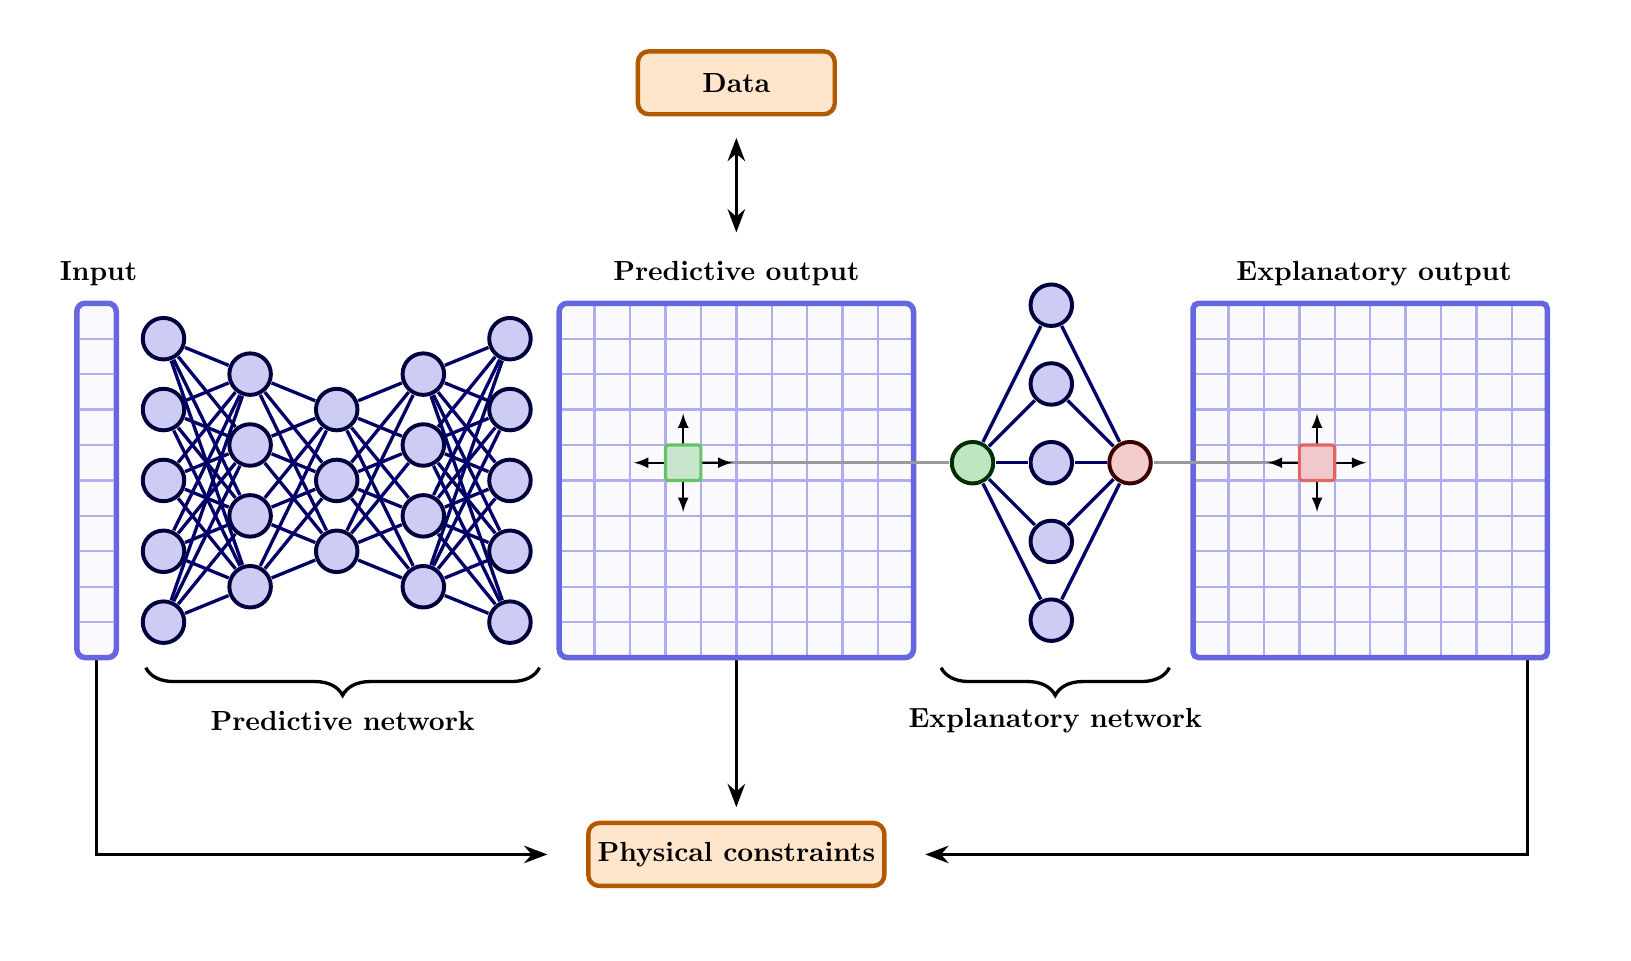
\begin{tikzpicture}
    \useasboundingbox (-0.5, -3.5) rectangle (19.5, 8);

    \draw[-Stealth, very thick, black] (0.37, 0) -| (0.37, -2.5) -> (6.1, -2.5); % From Input
    \draw[-Stealth, very thick, black] (8.5, 0) -| (8.5, -1.9); % From Predictive Output
    \draw[Stealth-Stealth, very thick, black] (8.5, 5.4) -- (8.5, 6.6); % From Predictive Output to Data
    \draw[-Stealth, very thick, black] (18.55, 0) -| (18.55, -2.5) -> (10.9, -2.5); % From Explanatory Output

    %=================== BOXES AND GRIDS ===================
    \draw [myblue!60, fill=myblue, fill opacity=0.02, rounded corners=3, line width=0.7mm] (0.125, 0.) --++ (0, 4.5) --++ (0.5, 0) --++ (0, -4.5) -- cycle;
    \foreach \i in {1,...,9} {\draw[myblue!30, line width=0.3mm] (0.16,  \i*0.45) -- (0.59, \i*0.45);}
    
    \foreach \i in {1,...,9} {
        \draw[myblue!30, line width=0.3mm] (6.25, \i*0.45) -- (10.75, \i*0.45);
        \draw[myblue!30, line width=0.3mm] (10.75 - \i*0.45, 0) -- (10.75 - \i*0.45, 4.5);}
    \draw [myblue!60, fill=myblue, fill opacity=0.02, rounded corners=3, line width=0.7mm] (6.25, 0) rectangle (10.75, 4.5);

    \foreach \i in {1,...,9} {
        \draw[myblue!30, line width=0.3mm] (16.0 - 1.7, \i*0.45) -- (20.5 - 1.7, \i*0.45);
        \draw[myblue!30, line width=0.3mm] (20.5 - 1.7 - \i*0.45, 0) -- (20.5 - 1.7 - \i*0.45, 4.5);}
    \draw [myblue!60, fill=myblue, fill opacity=0.02, rounded corners=2, line width=0.7mm] (14.3, 0) rectangle (20.5-1.7, 4.5);


    %=================== NEURAL NETWORKS ===================
    % --- Draw the Predictive Network ---
    \predictivenetwork{P}{5,4,3,4,5}{0.125}
    
    % --- Draw the Explanatory Network ---
    \explanatorynetwork{E}{1,5,1}{11.5}
    
    %=================== CONNECTIONS AND LABELS ===================
    \draw[black!40, very thick] (8.05, 2.25+0.45/2) -- (11.2, 2.25+0.45/2);
    \draw[->, thick] (8.05-0.45/2, 2.25+0.45) --++ (0, 0.4);
    \draw[->, thick] (8.05, 2.25+0.45/2) --++ (0.4, 0);
    \draw[->, thick] (8.05-0.45/2, 2.25) --++ (0, -0.4);
    \draw[->, thick] (8.05-0.45, 2.25+0.45/2) --++ (-0.4, 0);
    \draw[mygreen!60,fill=mygreen,fill opacity=0.2,rounded corners=1pt, line width=0.4mm] (8.05, 2.25) --++ (0, 0.45) --++ (-0.45, 0) --++ (0, -0.45) -- cycle;
    
    \draw[black!40, very thick] (13.8, 2.25+0.45/2) -- (16.1-0.45 , 2.25+0.45/2);
    \draw[->, thick] (16.1-0.45/2, 2.25+0.45) --++ (0, 0.4);
    \draw[->, thick] (16.1, 2.25+0.45/2) --++ (0.4, 0);
    \draw[->, thick] (16.1-0.45/2, 2.25) --++ (0, -0.4);
    \draw[->, thick] (16.1-0.45, 2.25+0.45/2) --++ (-0.4, 0);
    \draw[myred!60,fill=myred,fill opacity=0.2,rounded corners=1pt, line width=0.4mm] (16.1, 2.25) --++ (0, 0.45) --++ (-0.45, 0) --++ (0, -0.45) -- cycle;

    \draw[very thick, decorate, decoration={brace, amplitude=10pt, mirror, raise=2.5ex}]
      (1, 0.25) -- (6, 0.25) node[midway, yshift=-3em]{\textbf{Predictive network}};
    \draw[very thick, decorate, decoration={brace, amplitude=10pt, mirror, raise=2.5ex}]
      (11.1, 0.25) -- (14, 0.25) node[midway, yshift=-3em]{\textbf{Explanatory network}};

    \node[above, align=center, black!60!black] at (0.4, 4.6) {\textbf{Input}};
    \node[above, align=center, black!60!black] at (8.5, 4.6) {\textbf{Predictive output}};
    \node[above, align=center, black!60!black] at (16.6, 4.6) {\textbf{Explanatory output}};

     %=================== ADDITIONAL NODES ===================
    % 1. Create the "Physical constraints" node at the bottom
    \node[draw=orange!70!black, ultra thick, rounded corners, font=\bfseries, align=center, minimum width=2.5cm, minimum height=0.8cm, fill=orange!20] (constraints) at (8.5, -2.5) {\textbf{Physical constraints}};

    % 2. Create the "Data" node at the top
    \node[draw=orange!70!black, ultra thick, rounded corners, font=\bfseries, align=center, minimum width=2.5cm, minimum height=0.8cm, fill=orange!20] (data) at (8.5, 7.3) {\textbf{Data}};
    
\end{tikzpicture}
\end{document}